% Original author : Leslie Cheng
% Edited by Erik Gabrielsen
% For personal use only
%-------------------------------------

\documentclass[letterpaper,12pt]{article}[leftmargin=*]

\usepackage[empty]{fullpage}
\usepackage{enumitem}
\usepackage{ifxetex}
\ifxetex
  \usepackage{fontspec}
  \usepackage{hyperref}
\else
  \usepackage[utf8]{inputenc}
  \usepackage[T1]{fontenc}
  \usepackage[pdftex]{hyperref}
\fi
\usepackage{fontawesome}
\usepackage[sfdefault,light]{FiraSans}
\usepackage{anyfontsize}
\usepackage{xcolor}
\usepackage{tabularx}
\usepackage{graphicx}

%-------------------------------------------------- SETTINGS HERE --------------------------------------------------
% Header settings
\def \fullname {Erik Gabrielsen}
\def \subtitle {}

\def \linkedinicon {\faLinkedin}
\def \linkedinlink {http://www.linkedin.com/in/erik-gabrielsen-4505a6218}
\def \linkedintext {/erik-gabrielsen}

\def \phoneicon {\faPhone}
\def \phonetext {+47 960 45 058}

\def \emailicon {\faEnvelope}
\def \emaillink {mailto:erik.gabrielsen99@gmail.com}
\def \emailtext {erik.gabrielsen99@gmail.com}

\def \githubicon {\faGithub}
\def \githublink {https://github.com/dwight-schrute}
\def \githubtext {/dwight-schrute}

\def \websiteicon {\faGlobe}
\def \websitelink {https://google.com/}
\def \websitetext {dwightschrute.com}

\def \locationicon {\faMapMarker}
\def \locationtext {Neufelds gate 6, 7030 Trondheim}

\def \birthdayicon {\faBirthdayCake}
\def \birhtdaytext {21.12.1999}

\def \headertype {\headerphoto} % \singlecol or \doublecol

% Misc settings
\def \entryspacing {-0pt}

\def \bulletstyle {\faCaretRight}

% Define colours
\definecolor{primary}{HTML}{000000}
\definecolor{secondary}{RGB}{79, 100, 111}
\definecolor{accent}{HTML}{263238}
\definecolor{links}{HTML}{1565C0}

%------------------------------------------------------------------------------------------------------------------- 

% Defines to make listing easier
\def \linkedin {\href{\linkedinlink}{\linkedinicon}}
\def \phone {\phoneicon \hspace{3pt}{ \phonetext}}
\def \email {\emailicon \hspace{3pt}\href{\emaillink}{\emailtext}}
\def \github {\githubicon \hspace{3pt}\href{\githublink}{\githubtext}}
\def \website {\websiteicon \hspace{3pt}\href{\websitelink}{\websitetext}}
\def \location {\locationicon \hspace{3pt}{\locationtext} }
\def \birthday {\birthdayicon \hspace{3pt}{\birthdaytext} }

% Adjust margins
\addtolength{\oddsidemargin}{-0.55in}
\addtolength{\evensidemargin}{-0.55in}
\addtolength{\textwidth}{1.1in}
\addtolength{\topmargin}{-0.6in}
\addtolength{\textheight}{1.1in}

% Define the link colours
\hypersetup{
    colorlinks=true,
    urlcolor=links,
}

% Set the margin alignment 
\raggedbottom
\raggedright
\setlength{\tabcolsep}{0in}

%-------------------------
% Custom commands

% Sections
\renewcommand{\section}[2]{\vspace{5pt}
  \colorbox{secondary}{\color{white}\raggedbottom\normalsize\textbf{{#1}{\hspace{7pt}#2}}}
}

% Entry start and end, for spacing
\newcommand{\resumeEntryStart}{\begin{itemize}[leftmargin=2.5mm]\item[]}
\newcommand{\resumeEntryEnd}{\end{itemize}\vspace{\entryspacing}}

% Itemized list for the bullet points under an entry, if necessary
\newcommand{\resumeItemListStart}{\begin{itemize}[leftmargin=4.5mm]}
\newcommand{\resumeItemListEnd}{\end{itemize}}

% Resume item
\renewcommand{\labelitemii}{\bulletstyle}
\newcommand{\resumeItem}[1]{
  \item\small{
    {#1 \vspace{-2pt}}
  }
}

% Entry with title, subheading, date(s), and location
\newcommand{\resumeEntryTSDL}[4]{
  \vspace{-1pt}\item[]
    \begin{tabularx}{0.97\textwidth}{X@{\hspace{60pt}}r}
      \textbf{\color{primary}#1} & {\firabook\color{accent}\small#2} \\
      \textit{\color{accent}\small#3} & \textit{\color{accent}\small#4} \\
    \end{tabularx}\vspace{-6pt}
}

% Entry with title and date(s)
\newcommand{\resumeEntryTD}[2]{
  \vspace{-1pt}\item[]
    \begin{tabularx}{0.97\textwidth}{X@{\hspace{60pt}}r}
      \textbf{\color{primary}#1} & {\firabook\color{accent}\small#2} \\
    \end{tabularx}\vspace{-6pt}
}

% Entry for special (skills)
\newcommand{\resumeEntryS}[2]{
  \item[]\small{
    \textbf{\color{primary}#1 }{ #2 \vspace{-6pt}}
  }
}

% Double column header
\newcommand{\doublecol}[6]{
  \begin{tabularx}{\textwidth}{Xr}
    {
      \begin{tabular}[c]{l}
        \fontsize{35}{45}\selectfont{\color{primary}{{\textbf{\fullname}}}} \\
        {\textit{\subtitle}} % You could add a subtitle here
      \end{tabular}
    } & {
      \begin{tabular}[c]{l@{\hspace{1.5em}}l}
        {\small#4} & {\small#1} \\
        {\small#5} & {\small#2} \\
        {\small#6} & {\small#3}
      \end{tabular}
    }
  \end{tabularx}
}

% Single column header
\newcommand{\singlecol}[6]{
  \begin{tabularx}{\textwidth}{Xr}
    {
      \begin{tabular}[b]{l}
        \fontsize{35}{45}\selectfont{\color{primary}{{\textbf{\fullname}}}} \\
        {\textit{\subtitle}} % You could add a subtitle here
      \end{tabular}
    } & {
      \begin{tabular}[c]{l}
        {\small#1} \\
        {\small#2} \\
        {\small#3} \\
        {\small#4} \\
        {\small#5} \\
        {\small#6}
      \end{tabular}
    }
  \end{tabularx}
}

\newcommand{\headerphoto}[6]{
\begin{tabularx}{\textwidth}{Xr}
    {
      \begin{tabular}[b]{l}
        \fontsize{35}{45}\selectfont{\color{primary}{{\textbf{\fullname}}}} \\
        {\small#4 \quad \small#5} \\
        {\small \faBirthdayCake \hspace{3pt}21.12.1999 \quad \small \location \quad \linkedin}
      \end{tabular}
    } & {
      \begin{tabular}{l}
        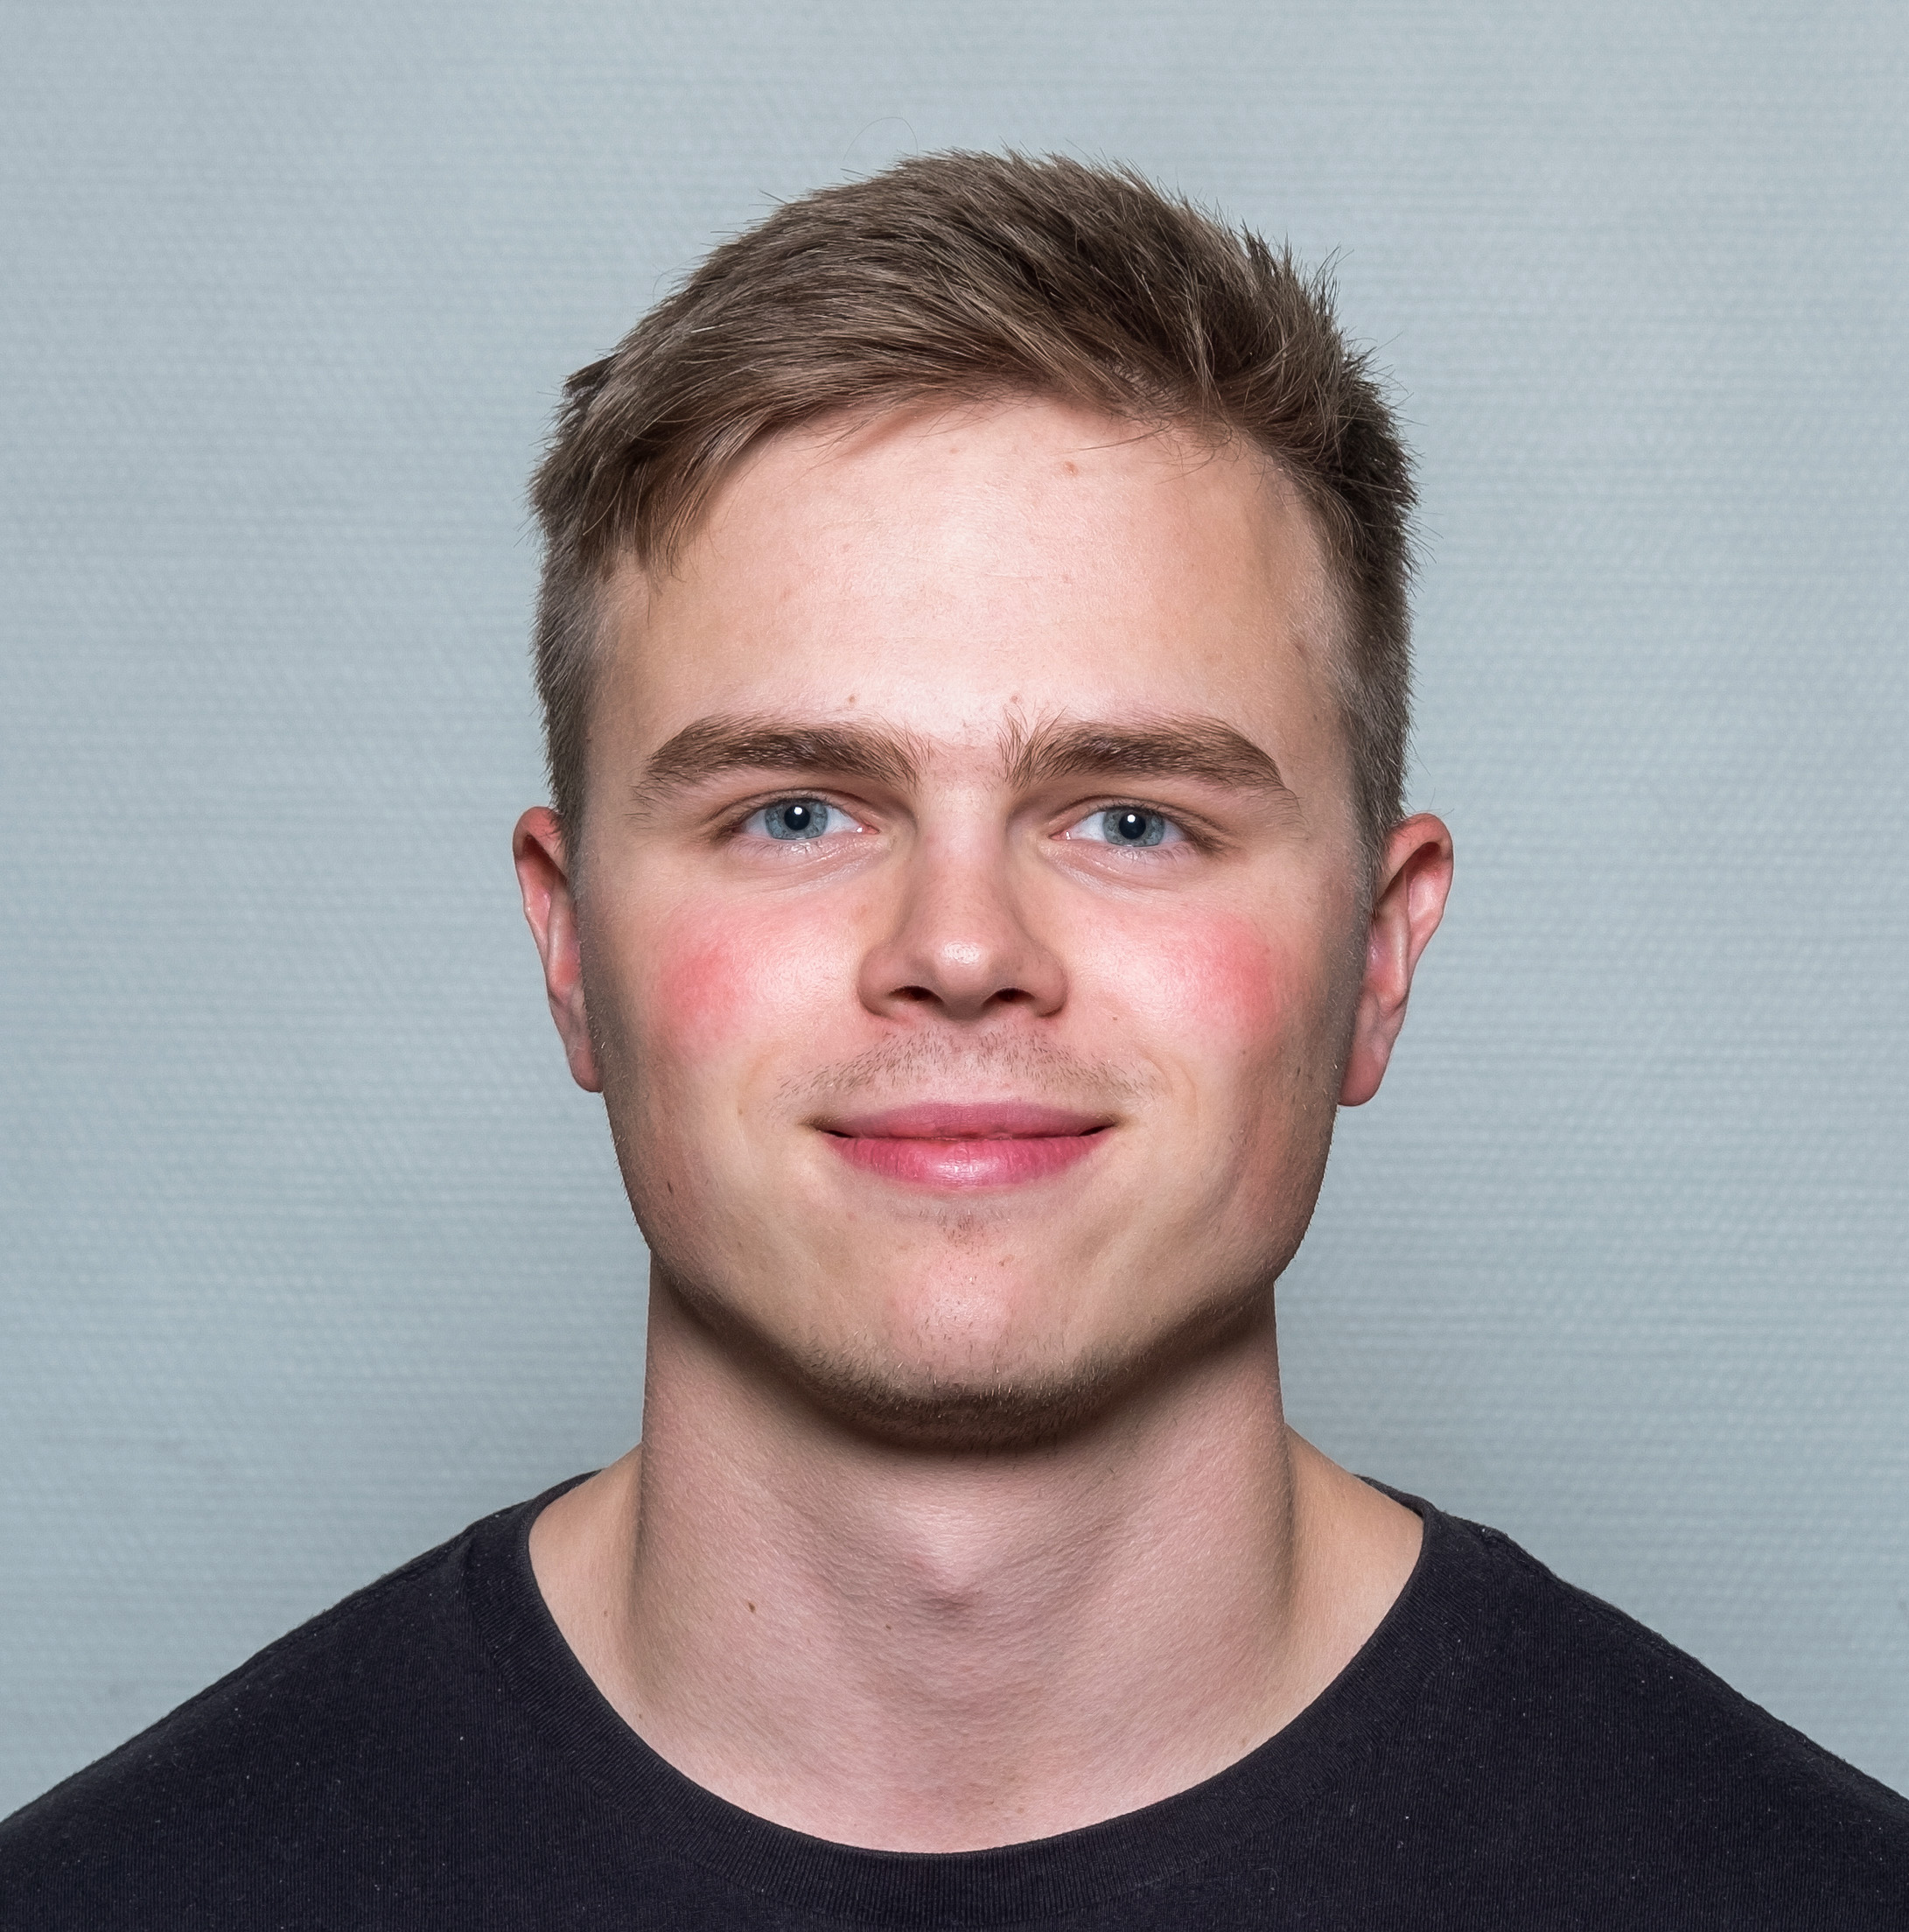
\includegraphics[width = 0.20\textwidth]{Erikg.jpg}
      \end{tabular}
    }
  \end{tabularx}
}

\begin{document}
%-------------------------------------------------- BEGIN HERE --------------------------------------------------

%---------------------------------------------------- HEADER ----------------------------------------------------
\headertype{\linkedin}{\github}{\website}{\phone}{\email}{} % Set the order of items here
\vspace{-50pt} % Set a negative value to push the body up, and the opposite

%-------------------------------------------------- EDUCATION --------------------------------------------------
\section{\faSendO}{Summary}

\resumeEntryStart
    \resumeItemListStart
      \resumeItem{Fifth year student of electronics systems design at NTNU.}
      \resumeItem{Extensive experience in UAV \& ROV hardware design.}
      \resumeItem{Concluded compulsory military service as a radio operator in the navy, and promoted to leading private.}
      \resumeItem{Combined five years of work experience and certificate of apprenticeship as a laboratory technician.}
    \resumeItemListEnd
\resumeEntryEnd

\section{\faGraduationCap}{Education}
\vspace{-10pt}
  \resumeEntryStart
    \resumeEntryTSDL
      {Electronic Systems Design \normalfont(MTELSYS)}{2020 -- now}
      {Norwegian University of Science and Technology}{Trondheim/Glasgow}
    
    \resumeEntryTSDL
    {The navy's radio operator course {\normalfont(CIS-1), as well as} fire fighting course}{2019}
    {Tordenskjold}{Bergen}
     
    \resumeEntryTSDL
    {Certificate of apprenticeship, Laboratory technician}{2019}
    {Elkem Technology}{Kristiansand}
    
    \resumeEntryTSDL
    {High school: Technical and general subjects \normalfont(TAF)}{2015 -- 2019}
    {Kvadraturen skolesenter}{Kristiansand}
  \resumeEntryEnd

\section{\faSuitcase}{Experience}
\vspace{-10pt}

  \resumeEntryStart
    \resumeEntryTSDL
    {Nortek}{Jun. 2024 -- Aug. 2024}
    {Summer internship}{Trondheim}
  \resumeItemListStart
    \resumeItem{Development of a sensor aquisition platform for an ROV.}
  \resumeItemListEnd
  \resumeEntryEnd

  \resumeEntryStart
    \resumeEntryTSDL
      {Kongsberg Defence \& Aerospace: LocalHawk}{Jun. 2023 -- Aug. 2023}
      {Summer internship}{Kongsberg}
    \resumeItemListStart
      \resumeItem {CAD and production of an energy efficient autonomous UAV using FDM and SLS printing technologies.}
    \resumeItemListEnd
  \resumeEntryEnd

  \resumeEntryStart
    \resumeEntryTSDL
      {Ascend NTNU}{Sep. 2022 -- Aug. 2023}
      {Hardware member}{Trondheim}
    \resumeItemListStart
      \resumeItem {Strategic role in design, development and testing of PCBs for use in UAVs in competition.}
      \resumeItem {Electronics and PCB design as main focus.}
    \resumeItemListEnd
  \resumeEntryEnd

  \resumeEntryStart
    \resumeEntryTSDL
      {Norwegian University of Science and Technology}{Jun. 2021 -- Aug. 2022}
      {Teaching assistant}{Trondheim}
    \resumeItemListStart
      \resumeItem {Part time employee at the IE faculty as a teaching assistant in the subject \textit{Introduction to Analog and Digital Electronics}.}
      \resumeItem {Employed the summers of 2021 and 2022 for further development of the subject.}
    \resumeItemListEnd
  \resumeEntryEnd

  \resumeEntryStart
    \resumeEntryTSDL
      {The Norwegian Navy}{Sep. 2019 -- Aug. 2020}
      {Radio Operator}{KNM Skjold}
    \resumeItemListStart
        \resumeItem {Operation, maintenance and administration of the vessel's communication stations.}
        \resumeItem {Promoted to leading private (ULM).}
    \resumeItemListEnd
  \resumeEntryEnd
\newpage
  \resumeEntryStart
    \resumeEntryTSDL
      {Elkem Technology}{Aug. 2015 -- Sep. 2019}
      {Apprentice, laboratory technician}{Kristiansand}
    \resumeItemListStart
      \resumeItem {Sample preparation, homogenisation and chemical analysis using a range of quantitative and qualitative analysis methods.}
    \resumeItemListEnd
  \resumeEntryEnd


%--------------------------------------------------Projects PROJECTS --------------------------------------------------
\section{\faPuzzlePiece}{Free time and volunteer work}
\vspace{-15pt}
  \resumeEntryStart
    \resumeEntryTD
      {Hardware member, Ascend}{2022 -- 2023}
    \resumeItemListStart
      \resumeItem {Ascend NTNU is an aerial robotics team consisting of students from the Norwegian University of Science and Technology.}
    \resumeItemListEnd
  \resumeEntryEnd
  \vspace{-1cm}
  \resumeEntryStart
    \resumeEntryTD
      {Volunteer in the brewing committee}{2020 -- 2022}
      \resumeItemListStart
        \resumeItem{Deputy leader.}
      \resumeItemListEnd
  \resumeEntryEnd
  \vspace{-1cm}
  \resumeEntryStart
    \resumeEntryTD
      {Some side projects include}{}
    \resumeItemListStart
      \resumeItem{Herb container with an automatic watering system.}
      \resumeItem{ATTINY85-based stop watch for use at the gym.}
      \resumeItem{Face recognition on the front door of the apartment.}
      \resumeItem{Photography as a hobby.}
    \resumeItemListEnd
  \resumeEntryEnd

  \section{\faUsers}{References}
  \vspace{-15pt}
  \resumeEntryStart
      \resumeEntryTSDL
        {Bjerknes, Jan Dyre -- \normalfont LocalHawk project supervisor}{907 02 187}
        {Senior Systems Engineer, Kongsberg Defence \& Aerospace}{}
  \resumeEntryEnd
  \resumeEntryStart
      \resumeEntryTSDL
        {Løvlie, John} {916 30 947}
        {Department manager - eWorks, Kongsberg Defence \& Aerospace}{}
  \resumeEntryEnd

  \resumeEntryStart
      \resumeEntryTSDL
        {Teisrud, Hege -- \normalfont Boss}{418 09 497}
        {Laboratory engineer, Elkem Technology}{}
  \resumeEntryEnd
  \resumeEntryStart
      \resumeEntryTSDL
        {Tefre, Joachim Lindholm -- \normalfont Training officer}{469 61 949}
        {Technician, KNM Skjold}{}
  \resumeEntryEnd

\end{document}